\section{Spindel Testen}

Momenteel worden de spindels die getest worden op de testkast alleen bekeken of deze draaien en of deze niet te veel trillen. De waardes hiervoor zijn niet bepaald en worden puur op gevoel getest. Het zou voor de klant maar ook voor Voortman best wat waarde kunnen hebben om ook echt waardes te hangen aan wat de motor maximaal mag trillen en bijvoorbeeld ook andere dingen te testen zoals de stroom die door de fasen van de motor gaat. Wanneer dit vervolgens in een testrapport komt van de motor kan er bewezen worden door Voortman dat de spindel weer goed is en weer juist werkt.

\subsection{Steekproef frequentie}

Veel testen op een elektro motor zijn gebaseerd op de volgende parameters:

\begin{enumerate}
	\item \textbf{Voltage}
	\item \textbf{Ampère}
	\item \textbf{Trillingen}
	\item \textbf{Temperatuur}
\end{enumerate}

Het voltage en de Ampère kunnen direct uitgelezen worden uit de drive. De \gls{AX5140} heeft een minimale sync cyclus tijd van 62,5 microseconden. Beckhoff \gls{PLC}’s ondersteunen cyclus tijden tot 50 microseconden mits de achterliggende \gls{PLC}-code niet te complex is waardoor de cyclus tijd niet gehaald kan worden. Dit zou betekenen dat er 16000 samples per seconde gemaakt kunnen worden wat weer zou betekenen dat de Nyquist frequentie 8000 is. Dit betekend dat er wat gezegd kan worden over frequenties tot 8000 Hz zonder dat er aliasing optreedt.

\vspace{0.5cm}

Trillingen kunnen niet standaard uitgelezen worden uit de drive en hiervoor moet zou daarom een extra sensor moeten komen zoals de MPB10 van SICK [8] die ook de motortemperatuur kan meten. Deze sensor moet echter aangesloten worden op een IO-Link terminal, deze terminals zijn vaak veel minder snel wat ten koste zou gaan van de Nyquist frequentie.

\newpage

\subsection{Fast Fourier Transformation}

Op veel meetgegevens worden bij het testen van een motor fourier transformaties uitgevoerd daarom wanneer dit vermeld staat in de komende testen wordt er het volgende bedoelt:

\vspace{0.5cm}

In de wiskunde converteert de discrete Fourier-transformatie (\gls{DFT}) een eindige reeks van op een gelijke afstand geplaatste reeks van samples in een reeks van even lange samples van dezelfde lengte van de discrete-time Fourier transformatie (\gls{DTFT}), wat een frequentiefunctie met complexe getallen is. De \gls{DFT} is een frequentiedomeinrepresentatie van de originele invoerreeks.


\begin{figure}[H]
	\centering
	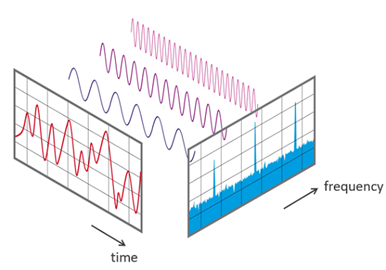
\includegraphics[width=300pt]{FourierTransform}
	\label{fig:FourierTransformatie}
	\caption{Fourier Transformatie \cite{web:FFT}}
\end{figure}

De formule van de \gls{DFT} is als volgt:

\begin{equation}
	X_k = \sum_{n=0}^{N-1}X_n e^{-i2\pi\frac{k}{N}n}
\end{equation}

Waarbij de complexiteit van de formule $O\left(N^2\right)$ is wat betekend dat een reeks van 1000 samples 1000000 berekeningen vereist om tot dezelfde reeks in het frequentiedomein te komen. Hierom is het verstandiger om een Cooley-Tukey FFT te gebruiken zoals het Radix-2 algoritme met complexiteit $O\left(Nlog{N}\right)$ die er als volgt uit ziet:

\begin{equation}
	X_k = {\sum_{m=0}^{\frac{N}{2}-1}X_{2m}e^{-\frac{2\pi i}{N}(2m)k}} + {\sum_{m=0}^{\frac{N}{2}-1}X_{2m+1}e^{-\frac{2\pi i}{N}(2m+1)k}}
\end{equation}

Het idee achter het Radix-2 algoritme is dat het eerst de even getallen berekend en daarna de oneven getallen waarna de 2 resultaten worden gecombineerd. Dit kan vervolgens recursief worden berekend. Met als enige eis dat de sample set grootte een macht van 2 is \cite{web:Radix-2FFT}.

\subsection{Rotorstang test}

Problemen in de rotorstang kunnen worden gevonden wanneer men kijkt naar de zijbanden van de pooldoorgangsfrequentie rond de lijnfrequentie kunnen deze duiden op problemen in de motor wanneer de motor onder belasting staat. De standaard regel is dat er een serieus probleem is wanneer de zijbandpieken binnen 35 \gls{dB} van de lijnfrequentiepiek komen. 

\vspace{0.5cm}

Met behulp van gedemoduleerde spannings- en stroom \gls{FFT}’s bij een hogere frequentie kunnen bijvoorbeeld problemen als dynamische en statische excentriciteit, losse rotorstaven en andere rotor gerelateerde fouten worden gedetecteerd \cite{web:MCSA}. 

\begin{figure}[H]
	\centering
	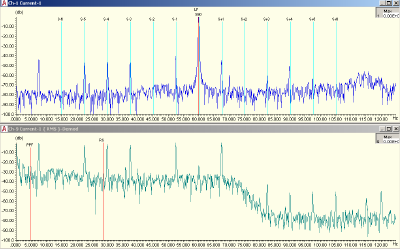
\includegraphics[width=300pt]{RotorStangTest}
	\label{fig:RotorStangTest}
	\caption{Pieken in de \gls{FFT} van de zijband \cite{web:MCSA}}
\end{figure}

\newpage

\subsection{Lager schade detectie doormiddel van trilling analyse}

Veel gevallen van motorstoringen komen door slijtage of schade aan de lager. Lager schade kan worden gedetecteerd door onder meer het trillen van de motor of spindel. Hierbij kan men bij de volgende vier frequentiepieken (door een \gls{FFT} uit te voeren op de trillingen) zien waar er schade aan de lager is.

\begin{figure}[H]
	\centering
	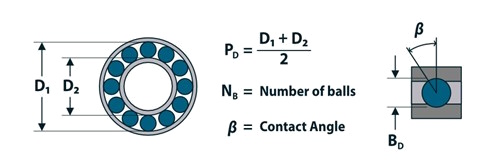
\includegraphics[width=300pt]{LagerSchade}
	\label{fig:LagerSchade}
	\caption{Lager schade herkennen door trillingen \cite{web:BearingFault}}
\end{figure}

\begin{itemize}
	\item \textbf{Balls Pass Frequency Outer Race (\gls{BPFO})} De \gls{BPFO}- of buitenringstoringsfrequentie komt overeen met het aantal kogels dat door een bepaald punt van de buitenring passeert elke keer als de as een volledige draai heeft gemaakt.
	
		\subitem 
			\begin{equation}
				BPFO = RPM\frac{N_b}{2}(1-\frac{B_D}{P_D}\cos\cos\beta)
			\end{equation}
	
	\item \textbf{Balls Pass Frequency Inner Race (\gls{BPFI})} De \gls{BPFI} of de binnenringstoringsfrequentie  komt overeen met het aantal kogels of rollen die door een bepaald punt van de binnenring passeert elke keer als de as een volledige draai heeft gemaakt.
	
		\subitem
			\begin{equation}
				BPFI = RPM\frac{N_b}{2}(1-\frac{B_D}{P_D}\cos \cos \beta)
			\end{equation}
			
	\item \textbf{Ball Spin Frequency (\gls{BSF})} De BSF- of rolelement storingsfrequentie komt overeen met het aantal omwentelingen dat een lager kogel of rol maakt elke keer wanneer de as een volledige draai heeft gemaakt.
	
		\subitem
			\begin{equation}
				BSF = RPM\frac{P_D}{B_D}[1-(\frac{B_D}{P_D} \cos \cos \beta)^2]
			\end{equation}
			
	\item \textbf{Fundamental Train Frequency (\gls{FTF})} De \gls{FTF} of kooistoringsfrequentie komt overeen met het aantal omwentelingen dat de lager kooi maakt elke keer wanneer de as een volledige draai heeft gemaakt.
	
		\subitem
			\begin{equation}
				FTF=RPM\frac{1}{2}(1-\frac{B_D}{P_D} \cos \cos \beta)
			\end{equation}
\end{itemize}

Indien er geen informatie beschikbaar is over de lagers dan kunnen 3 van de 4 frequenties toch empirisch worden berekend, waardoor de frequentie alleen nog maar afhankelijk is van het aantal rolelementen en de rotatiesnelheid.

\begin{equation}
	BPFO=0.4N_B RPM
\end{equation}

\begin{equation}
	BPFI=0.6N_B RPM
\end{equation}

\begin{equation}
	BPFI=0.4RPM
\end{equation}

Lager slijtage gaat vaak in verschillende fasen en heeft hierdoor invloed op de diagnoseprocedure. Lager defecten kunnen worden onderverdeeld in vier verschillende slijtagestadia. Het aantal trillingen neemt toe naarmate de lager in een hoger stadia komt. Het is daarom cruciaal om de problemen in een zo vroeg mogelijk stadium te detecteren en natuurlijk ook aan te pakken.

\begin{figure}[H]
	\centering
	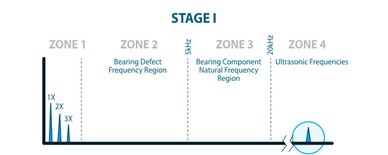
\includegraphics[width=\linewidth]{LagerStage1}
	\label{fig:LagerStage1}
	\caption{Stadia 1 \cite{web:BearingFault}}
\end{figure}

In het eerste stadia zijn er geen abnormale geluiden of temperatuurverschillen te zien. Echter kunnen er zich wel ultrasone geluiden vormen in de lager dit kunnen vroege waarschuwingen zijn dat de lager aan het slijten is.

\begin{figure}[H]
	\centering
	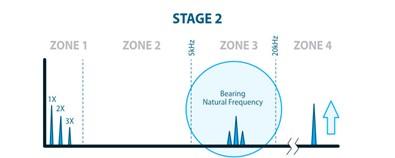
\includegraphics[width=\linewidth]{LagerStage2}
	\label{fig:LagerStage2}
	\caption{Stadia 2 \cite{web:BearingFault}}
\end{figure}

In het tweede stadia komen er meer ultrasone geluiden in de lager en er ontstaan ook hoge geluiden die wel te verstaan zijn door de mens vaak boven de 5kHz. Op dit moment moet er goed gelet worden op de lagers want deze hebben binnenkort onderhoudt nodig om ergere trillingen te voorkomen.

\begin{figure}[H]
	\centering
	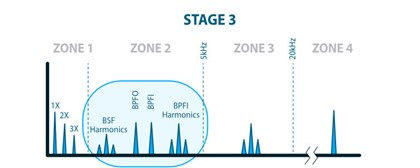
\includegraphics[width=\linewidth]{LagerStage3}
	\label{fig:LagerStage3}
	\caption{Stadia 3 \cite{web:BearingFault}}
\end{figure}

In het derde stadia blijven hoge frequenties opbouwen en ook de frequenties hierboven berekenend komen meer en meer in zicht. Wanneer een lager zich in dit stadia bevindt is het zeer verstandig om zo snel mogelijk de lager te vervangen.

\begin{figure}[H]
	\centering
	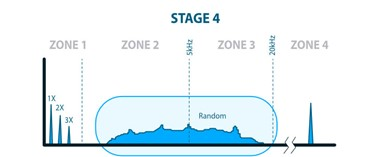
\includegraphics[width=\linewidth]{LagerStage4}
	\label{fig:LagerStage4}
	\caption{Stadia 4 \cite{web:BearingFault}}
\end{figure}

Stadia vier is het de laatste fase voordat de lager het helemaal zal begeven. Hoge frequenties zullen hier minder worden en ook de berekende frequenties die herkend konden worden zullen verdwijnen. Op dit moment zou een machine niet gebruikt mogen worden omdat de lager het hoogstwaarschijnlijk zal begeven binnenkort.

\newpage

\subsection{Rotor Excentriciteit}

De excentriciteit fouten tussen de rotor en de stator van een motor zorgen voor ongeveer 12\% tot 16\% van alle motor storingen \cite{MotorExcenttriciteit}. Er zijn hierbij twee varianten:

\begin{itemize}
	\item \textbf{Dynamische excentriciteit} hierbij veranderd de afstand tussen de stator en de rotor constant waardoor er onbalans en trillingen kunnen ontstaan. Oorzaken hiervan kunnen zijn versleten lagers, mechanische speling of een kromme rotorstang.
	
	\item \textbf{Statische excentriciteit} hierbij is de rotor niet in het midden geplaatst van de stator. De afstand tussen de rotor en stator is hierbij constant. Statische excentriciteit zal zorgen voor ongelijke magnetische krachten wat weer zal resulteren in extra energieverbruik en meer slijtage in de lagers.
\end{itemize}

\begin{figure}[H]
	\centering
	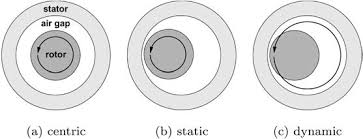
\includegraphics[width=\linewidth]{Excentricity}
	\label{fig:Excentricity}
	\caption{Motor excentriciteit \cite{staticdynamicexcentricity}}
\end{figure}

Bij excentriciteit kan men de volgende trillingen verwachten:

\begin{itemize}
	\item \textbf{Basisfrequentie van excentriciteit}
		\begin{equation}
			f_r=\frac{RPM}{60}
		\end{equation}
		
	\item \textbf{Harmonischen van de rotatiefrequentie} Statische en dynamische excentriciteit veroorzaken trillingen die een veelvoud zijn van de rotatie frequentie.
		\begin{equation}
			f_n=nf_r
		\end{equation}
\end{itemize}

\subsection{\gls{MCSA} (Motor Current Signature Analysis)}

Aan de hand van de motorstroom per fase van de motor kan men ook het een en ander zeggen over de staat van de motor. Zo kunnen afwijkingen in de stroom duiden op magneetschade, lager schade, slechte wikkelingen of op asymmetrie. Uit de AX5140 kan de stroom per fase gehaald worden en ook het voltage kan worden opgehaald uit de drive. Bij een inductie motor kunnen de pieken van de Fourier getransformeerde grafiek van het voltage en ampère worden vergeleken. Wanneer er een piek is in het voltage en ook bij de stroom dan is de fout van elektrische aart. Wanneer de piek alleen in de stroom zit dan is het probleem mechanisch \cite{web:MCSA}.

\begin{figure}[H]
	\centering
	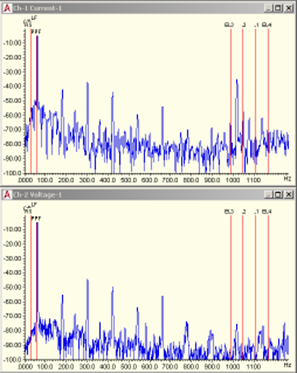
\includegraphics[width=0.5\linewidth]{MechanischeFout}
	\label{fig:MechanischeFout}
	\caption{Mechanische fout gevonden doormiddel van MCSA \cite{web:MCSA}}
\end{figure}

